\chapter{Interface Screenshots}

\begin{figure}[h!]
	\centering
	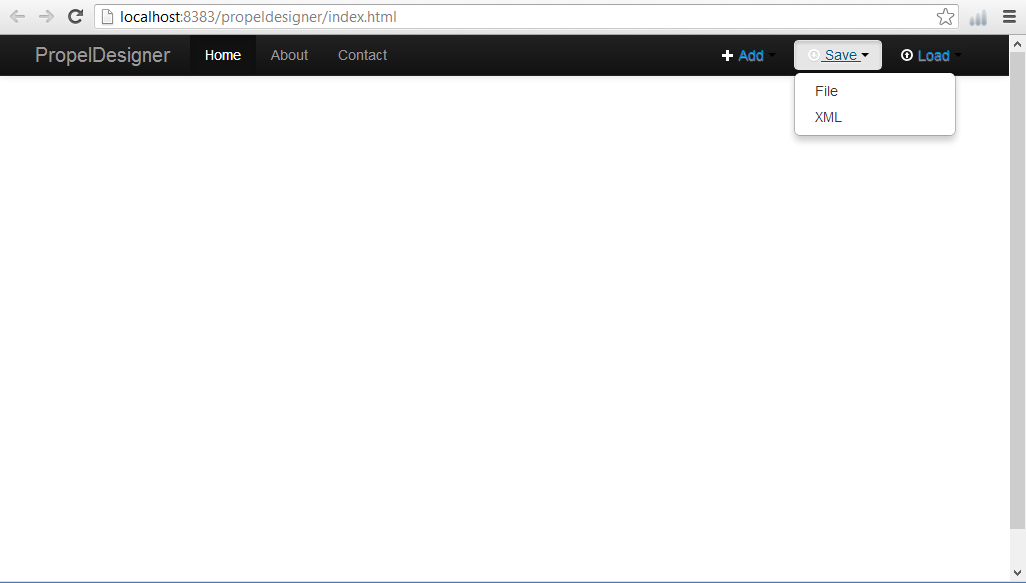
\includegraphics[width=15cm]{Images/blank_schema}
	\caption{This screen capture shows the SVG `canvas' in its initial, empty state. It also shows the UI features at the top of the screen and an example menu open.}
\end{figure}

\begin{figure}[h!]
	\centering
	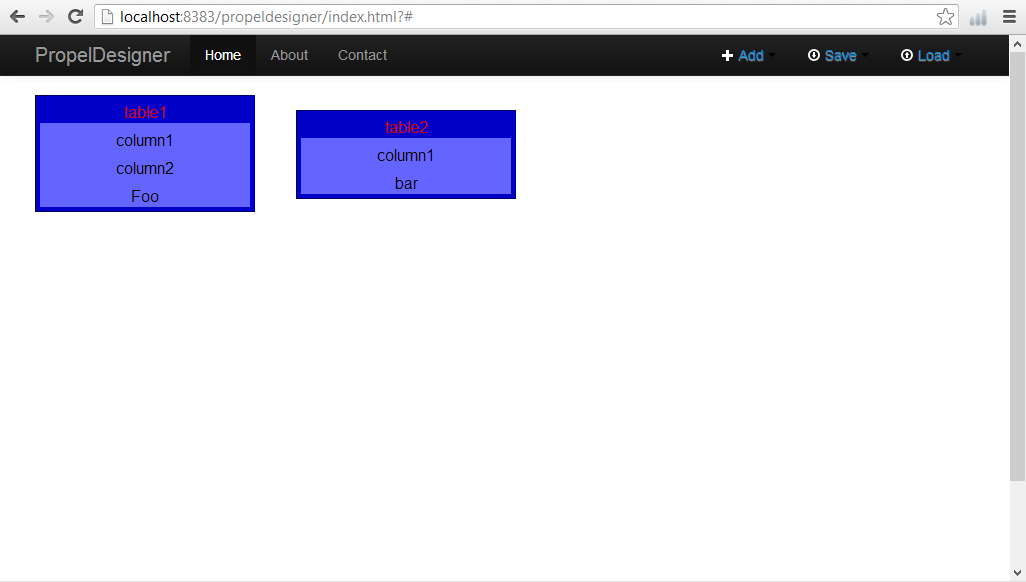
\includegraphics[width=15cm]{Images/populated_schema}
	\caption{This screen capture shows the SVG populated with two tables, each with a few columns. The colours are currently used to show to the developer the different parts of the SVG elements. The outermost rectangles (the tables) can be dragged around the SVG.}
\end{figure}

\begin{figure}[h!]
	\centering
	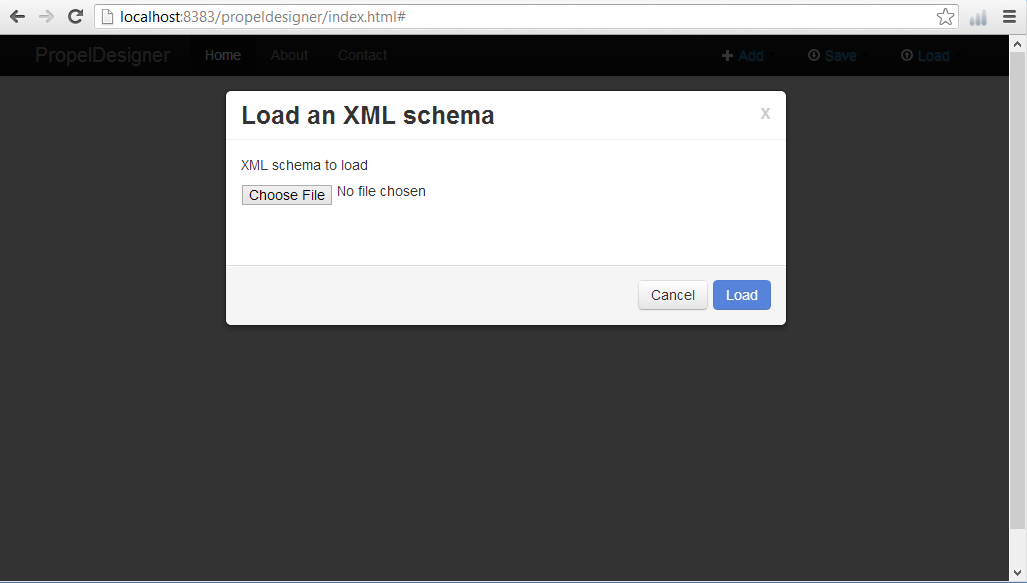
\includegraphics[width=15cm]{Images/open_file}
	\caption{This screen capture demonstrates the dialogue modal interface which, in this case, is showing the file load dialogue. The load button is disabled, here, as there is nothing to load.}
\end{figure}



\begin{figure}[h!]
	\centering
	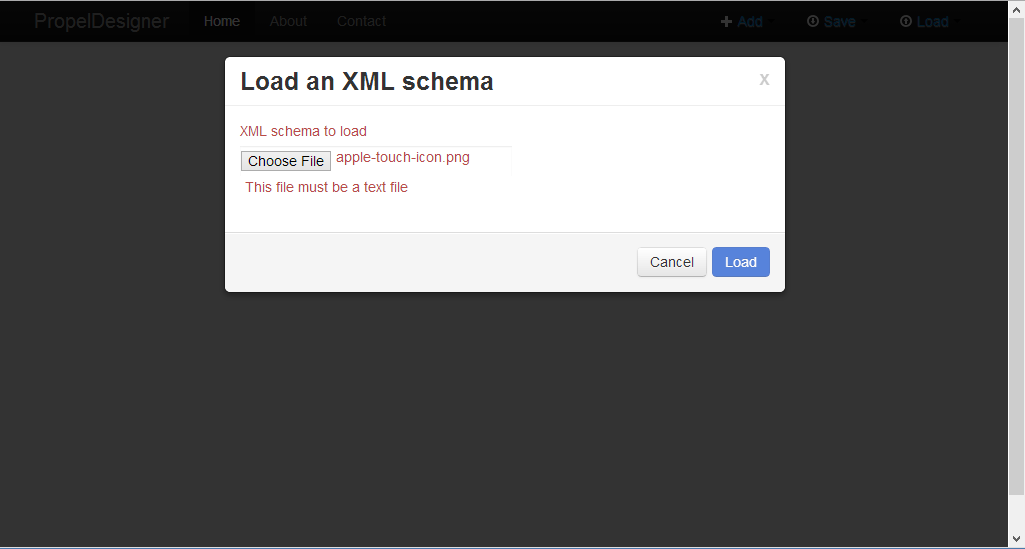
\includegraphics[width=15cm]{Images/open_error}
	\caption{This screen capture shows the previous screen capture, but where an incompatible file has been selected. This occurs without needing to load the file, using the File API in HTML5. The load button is still disabled. It will only become active when the file is of the text MIME type.}
\end{figure}